\documentclass[11pt]{article}

\usepackage[margin=1in]{geometry}
\usepackage{amsmath,amssymb}
\usepackage{booktabs}
\usepackage{enumitem}
\usepackage{pgfplots}
\pgfplotsset{compat=1.18}
\setlength{\parindent}{0pt}
\setlength{\parskip}{0.45em}

\begin{document}

\begin{enumerate}[label=\arabic*.,leftmargin=*,itemsep=1.5em]

\item \textbf{[10] (Looking back)}

Recall you (the Econ 532 class, Fall 2016) reported the number of trials ($X$)
needed to obtain the first head by tossing ``unbiased'' coins. A summary of
your data is given below:

\begin{center}
\begin{tabular}{lc}
\toprule
Value of $X$ & Observed Frequency \\
\midrule
1 & 14 \\
2 & 10 \\
3 & 6 \\
4 & 5 \\
5 or more & 5 \\
\midrule
Total & 40 \\
\bottomrule
\end{tabular}
\end{center}

Given these results, what would be a ``nice'' hypothesis to test? State your
null and alternative hypotheses and carry out an appropriate test.

\textit{Hint:} You may use the following Pearson $\chi^2$-test statistic:
\[
\chi_P^2=\sum_{j=1}^{r}\frac{(E_j-O_j)^2}{E_j},
\]
which approximately follows a $\chi^2_{r-1}$, where $E_j$ and $O_j$ are,
respectively, the expected and observed frequencies, and $r$ is the number
of classes or groups. $\chi^2_{0.05,5}=11.070$, and
$\chi^2_{0.05,4}=9.488$.

\item \textbf{[5 + 10 + 5] (The Great Expectations)}

A table of your expected midterm (Fall 2016) grade ($X$), observed grade
($Y$) (along with the scatter plot), and the difference ($Z=X-Y$) as
reported by thirty-eight (38) students is given below. Here the numbers
$1,2,3,4,5,6,7,8,$ and $9$ correspond to letter grades
$C-$, $C$, $C+$, $B-$, $B$, $B+$, $A-$, $A$, and $A+$, respectively.

\begin{enumerate}[label=(\roman*),leftmargin=2em]
\item Discuss the differences between $(\bar X,S_X^{\prime 2})$ and
$(\bar Y,S_Y^{\prime 2})$, if any.
\item Now we want to test $H_0:\mu_X=\mu_Y$. Write down your test
procedure, and interpret the result.
\item Now think about dividing the students into the top 50\% and the rest,
and testing the same hypothesis $H_0:\mu_X=\mu_Y$ separately for these
two groups. What would you expect? Discuss your answer without doing any
explicit calculations.
\end{enumerate}

\newpage
\begin{center}
\begin{minipage}[t]{0.38\linewidth}
\centering
\scriptsize
\renewcommand{\arraystretch}{0.82}
\begin{tabular}{lrrr}
\toprule
 & $X$ & $Y$ & $Z$ \\
\midrule
 & 9 & 9 & 0 \\
 & 9 & 6 & 3 \\
 & 9 & 7 & 2 \\
 & 9 & 8 & 1 \\
 & 9 & 7 & 2 \\
 & 8 & 7 & 1 \\
 & 8 & 9 & -1 \\
 & 8 & 9 & -1 \\
 & 8 & 5 & 3 \\
 & 8 & 8 & 0 \\
 & 7 & 6 & 1 \\
 & 7 & 9 & -2 \\
 & 7 & 8 & -1 \\
 & 7 & 8 & -1 \\
 & 7 & 4 & 3 \\
 & 7 & 3 & 4 \\
 & 6 & 8 & -2 \\
 & 6 & 6 & 0 \\
 & 6 & 6 & 0 \\
 & 6 & 6 & 0 \\
 & 6 & 6 & 0 \\
 & 6 & 6 & 0 \\
 & 5 & 3 & 2 \\
 & 5 & 5 & 0 \\
 & 5 & 7 & -2 \\
 & 5 & 5 & 0 \\
 & 5 & 6 & -1 \\
 & 4 & 8 & -4 \\
 & 4 & 7 & -3 \\
 & 4 & 2 & 2 \\
 & 4 & 7 & -3 \\
 & 3 & 5 & -2 \\
 & 3 & 3 & 0 \\
 & 3 & 6 & -3 \\
 & 2 & 5 & -3 \\
 & 2 & 3 & -1 \\
 & 2 & 3 & -1 \\
 & 1 & 2 & -1 \\
\midrule
Mean & $5.79$ & $6.01$ & $-0.21$ \\
Variance & $5.14$ & $4.11$ & $3.68$ \\
\bottomrule
\end{tabular}
\end{minipage}%
\hfill%
\begin{minipage}[t]{0.57\linewidth}
\centering
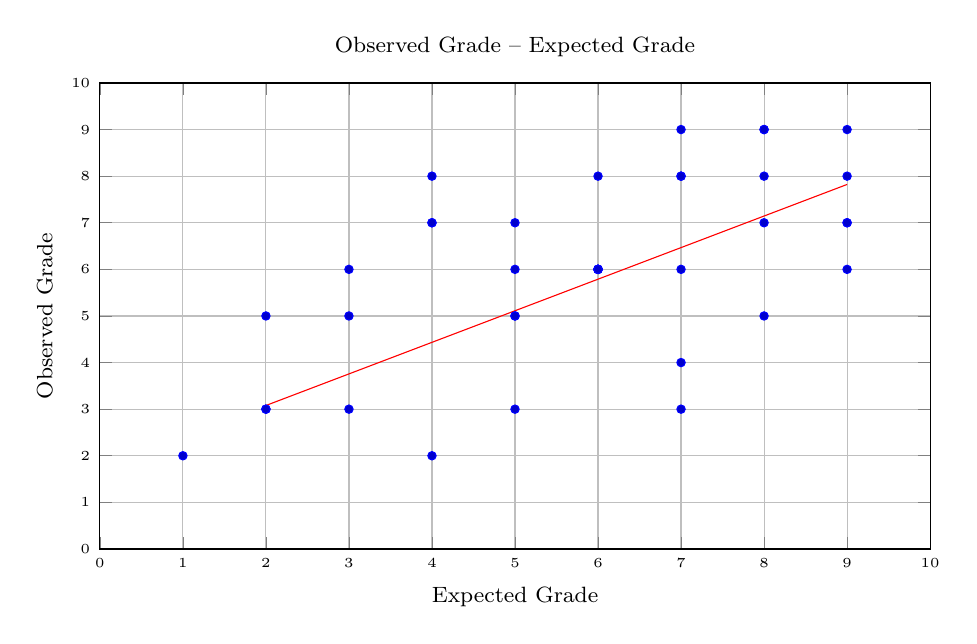
\begin{tikzpicture}
\begin{axis}[
    width=\linewidth,
    height=7.5cm,
    title={\footnotesize Observed Grade -- Expected Grade},
    xlabel={\footnotesize Expected Grade},
    ylabel={\footnotesize Observed Grade},
    xmin=0,xmax=10,ymin=0,ymax=10,
    xtick={0,...,10},ytick={0,...,10},
    grid=both,
    tick label style={font=\tiny},
    label style={font=\footnotesize},
    title style={font=\footnotesize},
]
\addplot+[only marks,mark=*,mark size=1.5pt] coordinates {
(9,9) (9,6) (9,7) (9,8) (9,7)
(8,7) (8,9) (8,9) (8,5) (8,8)
(7,6) (7,9) (7,8) (7,8) (7,4) (7,3)
(6,8) (6,6) (6,6) (6,6) (6,6) (6,6)
(5,3) (5,5) (5,7) (5,5) (5,6)
(4,8) (4,7) (4,2) (4,7)
(3,5) (3,3) (3,6)
(2,5) (2,3) (2,3) (1,2)
};
\addplot+[no marks,domain=2:9,samples=2] {0.6776*x+1.7237};
\end{axis}
\end{tikzpicture}

\vspace{0.75cm}
\raggedright
Formula used, for example:

Sample mean:
\[
\bar X=\frac{1}{n}\sum_{i=1}^{n}X_i.
\]

Sample variance:
\[
S_X^{\prime 2}=\frac{\sum_{i=1}^{n}(X_i-\bar X)^2}{n-1}.
\]
\end{minipage}
\end{center}

\newpage
\item \textbf{[15 + 10] (Asymptotics)}

\begin{enumerate}[label=(\roman*),leftmargin=2em]
\item If $g(\cdot)$ is a continuous function on the real line and
$X_n\xrightarrow{p}X$, then show that
$g(X_n)\xrightarrow{p}g(X)$.

\textit{Hint:} Use continuity of $g(\cdot)$: For a given $\varepsilon>0$,
there exists a $\delta>0$ such that
\[
|x_n-x|\leq\delta\ \Longrightarrow\
|g(x_n)-g(x)|<\varepsilon.
\]
\item Using the central limit theorem (CLT), show that
\[
\frac{\chi_n^2-n}{\sqrt{2n}}\xrightarrow{D}N(0,1).
\]
\end{enumerate}

\item \textbf{[25 + 5] (Some theory)}

\begin{enumerate}[label=(\roman*),leftmargin=2em]
\item Consider the MLE of $\theta$, $\hat\theta$. Using the result that
$\hat\theta\xrightarrow{p}\theta$, show
\[
\sqrt{n}(\hat\theta-\theta)\xrightarrow{D}
N\!\left(0,\frac{1}{\nu(\theta)}\right),
\]
where
\[
\nu(\theta)=
E\!\left[\left(\frac{d\log f(x,\theta)}{d\theta}\right)^2\right]
=E\!\left[-\frac{d^2\log f(x,\theta)}{d\theta^2}\right].
\]
In your proof you must state all the assumptions and results you use.

\textit{Hint:} Use the following Taylor series expansion:
\[
0=\left.\frac{1}{n}\frac{d\ell(\theta)}{d\theta}\right|_{\theta=\hat\theta}
=\frac{1}{n}\frac{d\ell(\theta)}{d\theta}
+\left.\frac{1}{n}\frac{d^2\ell(\theta)}{d\theta^2}\right|_{\theta=\theta^*}
(\hat\theta-\theta),
\]
where $\ell(\theta)$ is the log-likelihood function and $\theta^*$ lies
between the true value $\theta$ and $\hat\theta$.

\item Interpret the result in (i) in terms of efficiency of $\hat\theta$.
\end{enumerate}

\item \textbf{[15] (Testing/Tasting)}

Prove the Neyman--Pearson Lemma as given below:

A critical region $\omega_0$ of size $\alpha$ is most powerful if inside
$\omega_0$,
\[
\frac{L(\theta_0)}{L(\theta_a)}<k,
\]
and outside $\omega_0$,
\[
\frac{L(\theta_0)}{L(\theta_a)}\geq k,
\]
where $k$ is such that
\[
\Pr\!\left(\left.\frac{L(\theta_0)}{L(\theta_a)}<k\,\right|H_0\right)=\alpha.
\]

Notations are as used in class. However, you should explain the notations,
introduce new ones as needed, and state the required assumptions.

\item \textbf{[5 + 5] (Some Leading Personalities in Statistics who Influenced our Econ 532)}

Write a short note on the life and work of any one of the following
personalities:

\begin{itemize}[itemsep=0pt,topsep=0pt]
\item Karl Pearson
\item Prasanta Chandra Mahalanobis
\item Jerzy Neyman
\item David Blackwell
\item Calyampudi Radhakrishna Rao
\end{itemize}

\end{enumerate}

\end{document}
